\section{Removing Gradient Conflict: REPA-\texorpdfstring{$\Sigma$}{Sigma}}
\label{sec:repa_sigma}

The gradient-compatibility analysis of Section~\ref{sec:celeba} motivates a simple intervention.
We observed that the REPA gradient is well aligned with the diffusion gradient at high noise levels but becomes
\emph{anticorrelated} at low noise levels and late in training (Figure~\ref{fig:grad_compat}). In that regime the
auxiliary term actively pulls the update against the direction that decreases the diffusion loss, so a constant
alignment weight $\lambda$ eventually does more harm than good. Rather than switching the alignment loss off entirely,
as proposed by~\cite{wang2025haste}, we keep the part of the REPA gradient that helps and discard only the part that
conflicts. We call the resulting gradient adapter \emph{REPA-$\Sigma$}.

\paragraph{The REPA-\texorpdfstring{$\Sigma$}{Sigma} adapter.}
At a training step with weights $w$, let
\[
  g \;=\; \nabla_w \mathcal{L}_{\mathrm{diff}}, \qquad
  r \;=\; \nabla_w \mathcal{L}_{\mathrm{REPA}}
\]
be the diffusion and REPA gradients. As a low-variance reference for the primary descent direction we use
$\bar g$, an estimate of the diffusion gradient evaluated at the exponential-moving-average (EMA) weights $\bar w$
that are already maintained for sampling. Vanilla REPA forms the update direction $g + \lambda r$. REPA-$\Sigma$ instead
replaces $r$ with its conflict-free counterpart, removing only the component of $r$ that is \emph{anti}-aligned with
$\bar g$:
\begin{equation}
  r^{\Sigma}
  \;=\;
  r \;-\; \frac{\big[\langle r, \bar g\rangle\big]_{-}}{\|\bar g\|_2^2}\,\bar g,
  \qquad
  [x]_{-} \;=\; \min(x, 0),
  \label{eq:repa_sigma}
\end{equation}
and uses the update direction $u_{\Sigma} = g + \lambda\, r^{\Sigma}$. When $\langle r,\bar g\rangle \ge 0$ the bracket
vanishes and $r^{\Sigma}=r$, so aligned REPA gradients pass through untouched. When $\langle r,\bar g\rangle < 0$ the
adapter subtracts exactly the offending projection, leaving $r^{\Sigma}$ orthogonal to $\bar g$. The operation is
parameter-free and adds only one inner product and one axpy per step.

\subsection{General Theoretical Results}
\label{sec:repa_sigma_theory}

We formalise the two properties that make \eqref{eq:repa_sigma} a safe modification of the auxiliary gradient.

\paragraph{Minimal change.}
The adapted gradient $r^{\Sigma}$ is the closest vector to $r$ that does not conflict with the reference direction:
\[
  r^{\Sigma}
  \;=\;
  \operatorname*{arg\,min}_{r'} \ \tfrac{1}{2}\|r' - r\|_2^2
  \quad \text{s.t.} \quad
  \langle r', \bar g\rangle \ge 0 .
\]
That is, $r^{\Sigma}$ is the Euclidean projection of $r$ onto the half-space $\{r' : \langle r', \bar g\rangle \ge 0\}$,
so REPA-$\Sigma$ alters the alignment signal as little as possible while eliminating the conflict.

\paragraph{Guaranteed non-interference.}
By construction $\langle r^{\Sigma}, \bar g\rangle = \big[\langle r, \bar g\rangle\big]_{+} \ge 0$, where
$[x]_{+}=\max(x,0)$. Hence for every $\lambda \ge 0$,
\[
  \langle u_{\Sigma}, \bar g\rangle
  \;=\;
  \langle g, \bar g\rangle + \lambda\,\big[\langle r, \bar g\rangle\big]_{+}
  \;\ge\;
  \langle g, \bar g\rangle .
\]
Adding the adapted alignment gradient therefore never decreases the inner product with the primary descent direction,
whereas the vanilla direction $g + \lambda r$ satisfies $\langle g+\lambda r, \bar g\rangle = \langle g,\bar g\rangle +
\lambda\langle r,\bar g\rangle$, which can fall below $\langle g,\bar g\rangle$ -- and even become negative -- once
$\lambda\langle r,\bar g\rangle$ is sufficiently negative. In the idealised case where the reference is exact
($\bar g = g$), a gradient-flow step gives
\[
  \frac{d}{dt}\,\mathcal{L}_{\mathrm{diff}}
  \;=\;
  -\langle g, u_{\Sigma}\rangle
  \;=\;
  -\|g\|_2^2 \;-\; \lambda\,\big[\langle g, r\rangle\big]_{+}
  \;\le\; -\|g\|_2^2 \;\le\; 0,
\]
so the diffusion loss decreases at least as fast as pure diffusion training for any $\lambda$, while still absorbing the
auxiliary gradient whenever it is aligned. Under the vanilla objective the same quantity is $-\|g\|_2^2 -
\lambda\langle g,r\rangle$, which is \emph{positive} -- i.e.\ the diffusion loss momentarily increases -- whenever
$\lambda\langle g,r\rangle < -\|g\|_2^2$. This is exactly the late-training, low-noise regime identified in
Figure~\ref{fig:grad_compat}.

\subsection{Toy Model}

\subsubsection{Problem setting}

\subsubsection{Some theory}

\subsubsection{Experiments}

\subsection{CelebA Results}
\label{sec:repa_sigma_celeba}

We validate the adapter on the CelebA setup of Section~\ref{sec:celeba}, comparing five configurations along two
independent axes -- gradient surgery (REPA vs.\ REPA-$\Sigma$) and a linear annealing schedule for the alignment weight
$\lambda$: the diffusion baseline, REPA with constant $\lambda$, REPA-$\Sigma$ with constant $\lambda$, and the
$\lambda$-annealed versions of both. All models share architecture, optimiser, data, and compute budget; only the
treatment of the alignment gradient differs.

\begin{figure}
  \centering
  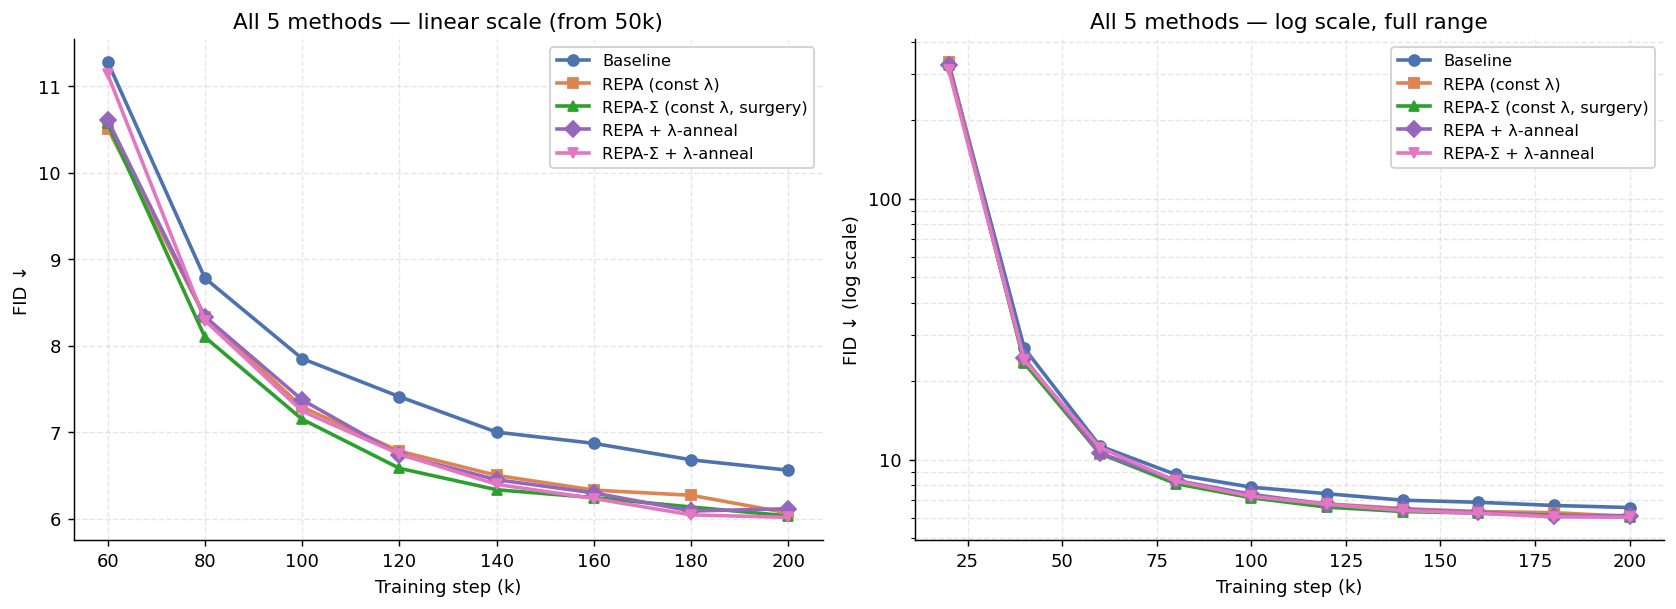
\includegraphics[width=\linewidth]{images/fid_5_methods.png}
  \caption{FID versus training step for the five configurations on CelebA. Left: linear scale from 50\,k steps;
  right: log scale over the full range. Every REPA variant converges faster than the diffusion baseline, and the
  REPA-$\Sigma$ variants track or slightly improve on vanilla REPA throughout training.}
  \label{fig:fid_5_methods}
\end{figure}

\begin{figure}
  \centering
  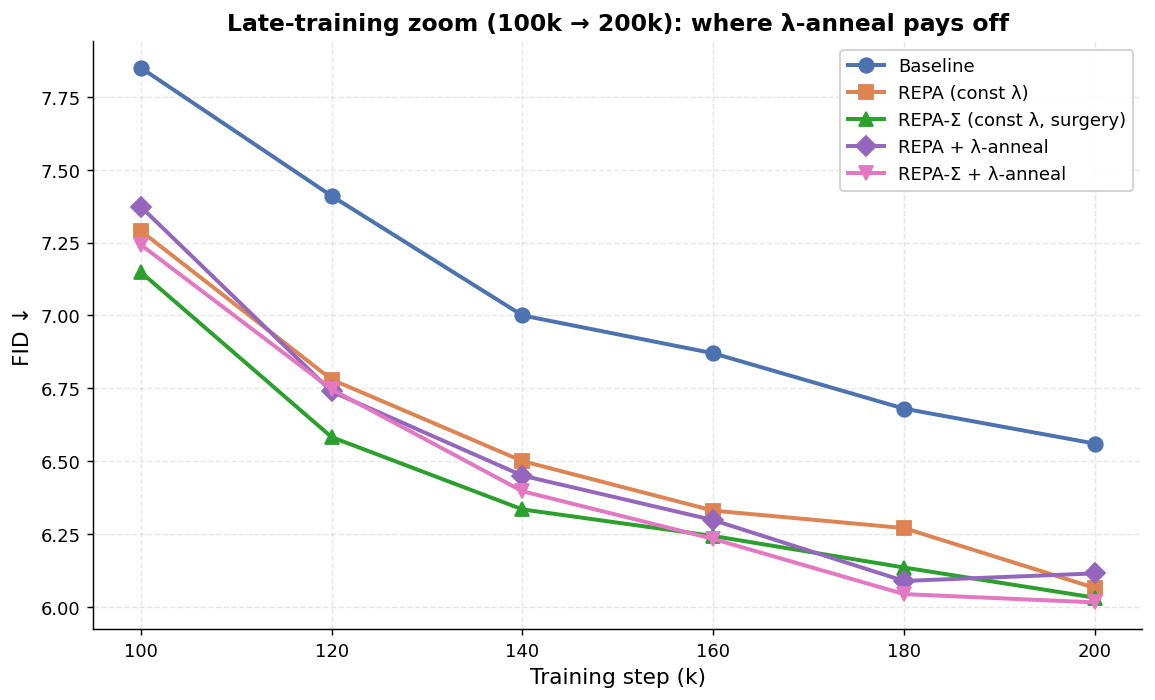
\includegraphics[width=0.85\linewidth]{images/fid_100k_200k.png}
  \caption{Late-training zoom (100\,k\,$\rightarrow$\,200\,k steps) on CelebA. Gradient surgery (REPA-$\Sigma$) gives
  the largest gains in the 100\,k--160\,k window, while annealing $\lambda$ pays off near the end of training; the two
  effects combine, with REPA-$\Sigma$ $+\ \lambda$-anneal reaching the lowest final FID.}
  \label{fig:fid_late}
\end{figure}

Figure~\ref{fig:fid_5_methods} shows the full FID trajectories: all four representation-alignment variants converge
substantially faster than the diffusion baseline, and the REPA-$\Sigma$ curves match or modestly improve on vanilla
REPA across the whole run. The differences among the alignment variants are best seen in the late-training zoom of
Figure~\ref{fig:fid_late}. Two complementary effects emerge. First, the gradient surgery itself is most valuable in the
\emph{middle} of training (roughly 100\,k--160\,k steps), where REPA-$\Sigma$ with constant $\lambda$ attains the lowest
FID -- consistent with the theory, since this is the window in which the conflicting low-noise component starts to
dominate while the alignment weight is still large. Second, \emph{annealing} $\lambda$ pays off \emph{late}: in the
final 180\,k--200\,k steps the annealed variants overtake their constant-$\lambda$ counterparts. The two mechanisms are
complementary, and combining them -- REPA-$\Sigma$ with $\lambda$ annealing -- yields the best final quality, reaching
$\mathrm{FID}\approx 6.0$ at 200\,k steps versus $\approx 6.1$ for vanilla REPA and $\approx 6.6$ for the baseline.
Overall, removing the anticorrelated component of the REPA gradient is a cheap, theoretically grounded modification that
never hurts and provides a small but consistent improvement over standard representation alignment, especially when
paired with a decaying alignment weight.
